\documentclass [aspectratio=169]{beamer}
\beamertemplatenavigationsymbolsempty
\usetheme{Boadilla}
\usepackage{textpos} % package for the positioning
\usepackage[]{graphicx}
\usepackage{graphicx}
\usepackage{float}
\usepackage{hyperref}
\usepackage{caption}
\usepackage{subcaption}
\usepackage{algorithm,algpseudocode}
\usepackage[export]{adjustbox}
\usepackage{tikz}
\usepackage[square,numbers]{natbib}
\usepackage[byname]{smartref}
\usetikzlibrary{positioning}
\usetikzlibrary{arrows, shapes, decorations, automata, backgrounds, fit, petri, calc}

\newcommand*{\logofont}{\fontfamily{phv}\selectfont}

\definecolor{uwopurple}{RGB}{79,38,131} % official purple color for uwo

\title[]{\vspace{60pt} \\
Liquid Times} % Change the lecture topic right here!
\subtitle{The nEXO way}
\author[]{J.J. Gómez Cadenas}
\institute[]{Donostia International Physics Center}
\date{\today}

% Math notations
\newtheorem{thm}{Theorem}[section]
\newtheorem{lem}[thm]{Lemma}

\newtheorem{defn}[thm]{Definition}
\newtheorem{eg}[thm]{Example}
\newtheorem{ex}[thm]{Exercise}
\newtheorem{conj}[thm]{Conjecture}
\newtheorem{cor}[thm]{Corollary}
\newtheorem{claim}[thm]{Claim}
\newtheorem{rmk}[thm]{Remark}

\newcommand{\ie}{\emph{i.e.} }
\newcommand{\cf}{\emph{cf.} }
\newcommand{\into}{\hookrightarrow}
\newcommand{\dirac}{\slashed{\partial}}
\newcommand{\bbonu}{\ensuremath{\beta\beta0\nu}}
\newcommand{\bbtnu}{\ensuremath{\beta\beta2\nu}}
\newcommand{\mbb}{\ensuremath{m_{\beta\beta}}}
\newcommand{\qbb}{\ensuremath{Q_{\beta\beta}}}
\newcommand{\mbbsq}{\ensuremath{m_{\beta\beta}^2}}
\newcommand{\tonu}{\ensuremath{(T_{1/2}^{0\nu})^{-1}}}
\newcommand{\gonu}{\ensuremath{G^{0\nu}}}
\newcommand{\monu}{\ensuremath{| M^{0\nu}|^2}}
\newcommand{\XE}{\ensuremath{{}^{136}{\rm Xe}}}
\newcommand{\XES}{\ensuremath{{}^{137}{\rm Xe}}}
\newcommand{\GE}{\ensuremath{{}^{76}{\rm Ge}}}
\newcommand{\TE}{\ensuremath{{}^{130}{\rm Te}}}
\newcommand{\TL}{\ensuremath{{}^{208}{\rm Tl}}}
\newcommand{\BI}{\ensuremath{{}^{214}{\rm Bi}}}
\newcommand{\MO}{\ensuremath{{}^{100}{\rm Mo}}}
\newcommand{\KR}{\ensuremath{{}^{83}{\rm Kr}}}
\newcommand{\nne}{\ensuremath{\bar{N}_e}}
\newcommand{\nng}{\ensuremath{\bar{N}_\gamma}}
\newcommand{\so}{\ensuremath{\rm S_1}}
\newcommand{\st}{\ensuremath{\rm S_2}}
\newcommand{\tz}{\ensuremath{\rm t_0}}
\newcommand{\R}{\mathbb{R}}
\newcommand{\C}{\mathbb{C}}
\newcommand{\Z}{\mathbb{Z}}
\newcommand{\N}{\mathbb{N}}
\newcommand{\Q}{\mathbb{Q}}
\newcommand{\LieT}{\mathfrak{t}}
\newcommand{\T}{\mathbb{T}}
\newcommand{\A}{\mathds{A}}
\newcommand{\E}{\mathbb{E}}
\newcommand{\Prob}{\mathbb{P}}
\newcommand{\Var}{\text{Var}}
\newcommand\equalhat{%
\let\savearraystretch\arraystretch
\renewcommand\arraystretch{0.3}
\begin{array}{c}
\stretchto{
    \scalerel*[\widthof{=}]{\wedge}
    {\rule{1ex}{3ex}}%
}{0.5ex}\\ 
=%
\end{array}
\let\arraystretch\savearraystretch
}

% set color
\setbeamercolor{title in head/foot}{bg=white}
\setbeamercolor{author in head/foot}{bg=white}
\setbeamercolor{date in head/foot}{fg=uwopurple}
\setbeamercolor{date in head/foot}{bg=white}
\setbeamercolor{title}{fg=uwopurple}
\setbeamerfont{title}{series=\bfseries}
\setbeamercolor{frametitle}{fg=uwopurple}
\setbeamerfont{frametitle}{series=\bfseries}
\setbeamercolor{block title}{bg=uwopurple!30,fg=black}
\setbeamercolor{item}{fg=uwopurple}
\setbeamercolor{caption name}{fg=uwopurple!70!}


% set logo at non-title pages
%\logo{
\includegraphics[height=0.9cm]{dipc.png}\vspace*{-.45\paperheight}\hspace*{.50\paperwidth}}

\begin{document}

{
\setbeamertemplate{logo}{}
\begin{frame}
    \titlepage
    \begin{textblock*}{4cm}(0.5cm,-7.3cm)
        
\includegraphics[width=4cm]{dipc.png}
    \end{textblock*}
    \begin{textblock*}{8cm}(5.0cm,-7.0cm)
        \huge \color{uwopurple}{$\Bigr\rvert$ \hspace{0.15cm} \textbf{Lecture 6}} % Change the lecture # right here! 
    \end{textblock*}
\end{frame}
}

%%%%
\begin{frame}{The LXe (single phase) TPC}
\begin{columns}
\column{0.50\textwidth}
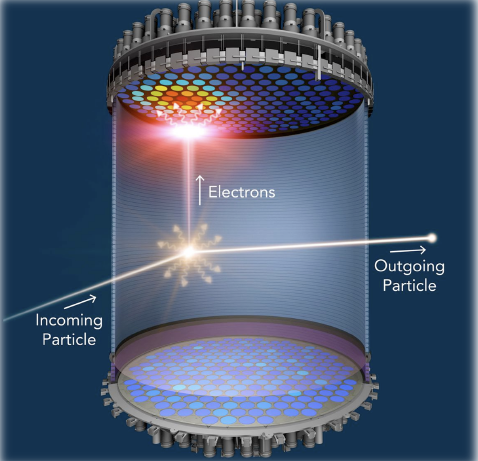
\includegraphics[scale=0.26]{dualLXe.png}

$\bullet~$ {\bf Two-phase LXe-TPC}: same principle that the HPXe TPC (NEXT). Reads primary scintillation (\so) and a delayed secondary scintillation (\st) produced by EL amplification (in gas). 

\column{0.50\textwidth}
 \begin{textblock*}{8cm}(0.5cm, -3.4cm)
 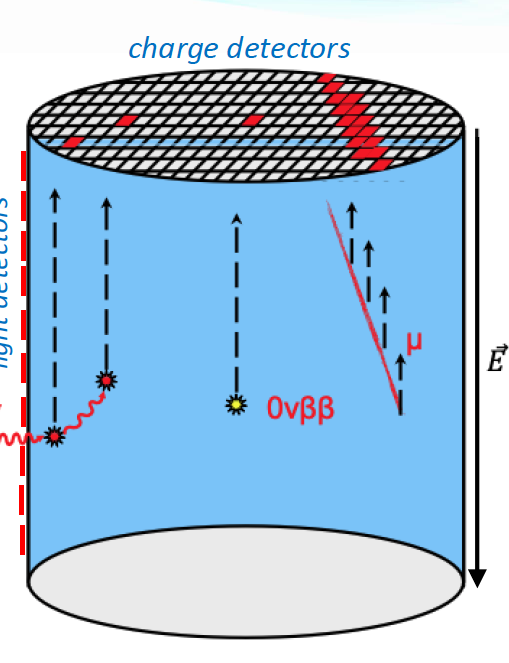
\includegraphics[scale=0.20]{nexobasis.png}
       % 
\includegraphics[width=4cm]{dipc.png}
       
       $\bullet~$ {\bf Single-phase LXe-TPC}: Reads primary scintillation (\so) and collects the ionisation charge in wires (no EL amplification). 

    \end{textblock*}


%$\bullet~$ {\bf Single-phase LXe-TPC}: Reads primary scintillation (\so) and collects the ionisation charge in wires (no EL amplification). 


%64,000 e/MeV 

%Q = E/W, W=15.6 eV. (13.8 at zero drift field). 

\end{columns}
\end{frame}

\begin{frame}{The LXe (single phase) TPC}
\begin{columns}
\column{0.50\textwidth}
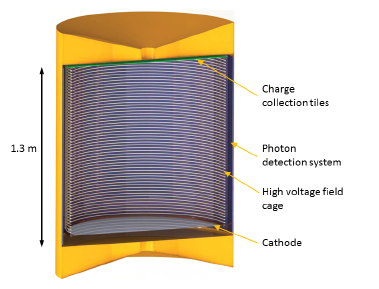
\includegraphics[scale=0.6]{nexosketch.png}

\column{0.50\textwidth}
$\bullet~$ {\bf Single-phase advantages}: simplicity, resulting in fewer components and lower background. 

$\bullet~$ {\bf Single-phase disadvantages}: no amplification of \st, thus higher threshold. Thus, \KR\ calibration no possible (but there are other possibilities). At 2.5 MeV, $Q = 2.5\times 10^6/15.6 = 160\, 256$~electrons, enough to measure the charge with good resolution.  
\end{columns}
\end{frame}

\begin{frame}{The LXe (asymmetric) TPC}
\begin{columns}
\column{0.50\textwidth}
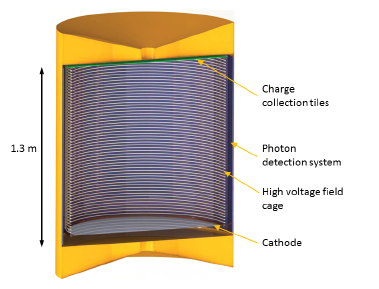
\includegraphics[scale=0.6]{nexosketch.png}

\column{0.50\textwidth}
$\bullet~$ {\bf asymmetric advantage}: Grids (thus radon decays) in the edges of the fiducial volume (unlike the case of NEXT, where the gas is rather transparent, this is a must, otherwise shielding inefficient). 

$\bullet~$ {\bf asymmetric disadvantages}: Double drift distance and potencial at the cathode.  
\end{columns}
\end{frame}

\begin{frame}{The LXe (instrumented barrel) TPC}
\begin{columns}
\column{0.50\textwidth}
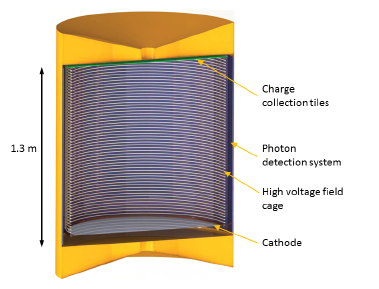
\includegraphics[scale=0.6]{nexosketch.png}

\column{0.50\textwidth}
$\bullet~$ {\bf advantage}: Avoid PMTs which are rather radioactive (same argument for NEXT). 

$\bullet~$ {\bf disadvantage}: Lots of SiPMs!. 

$\bullet~$ {\bf Exercise}: Why not a BFD like NEXT-HD?  
\end{columns}
\end{frame}
%%%%

\begin{frame}{Gamma attenuation in LXe}
\begin{columns}
\column{0.50\textwidth}
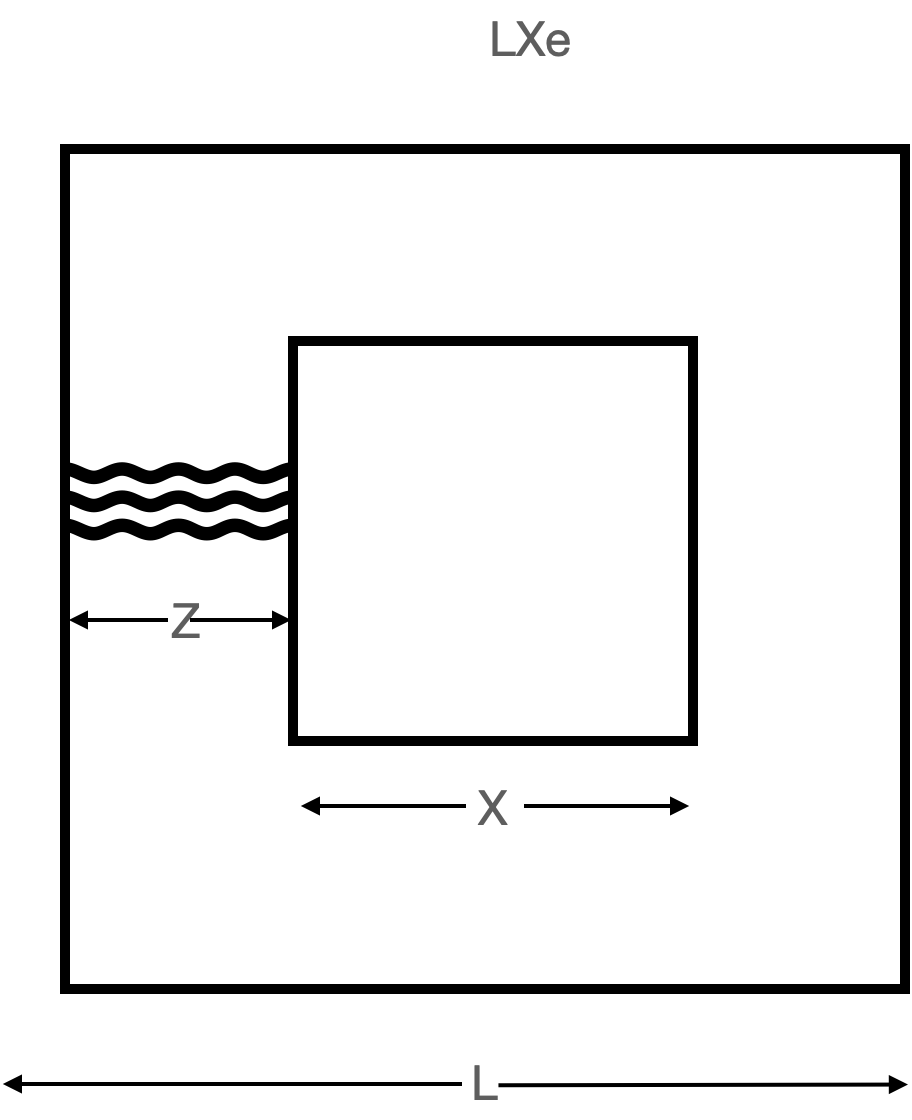
\includegraphics[scale=0.2]{attLxe.png}

$\bullet~$ Consider a LXe TPC with $L = 125$~ cm and $D = 116$~ cm (e.g, similar to nEXO). It will host 4.1 tons of LXe.

$\bullet~$ Define a fiducial region as a volume, centred in the TPC of 
$l = 86$~ cm and $d = 71$~ cm. It will host $\sim$1 ton of LXe

\column{0.50\textwidth}
$\bullet~$ The shielding length for gammas emitted from the end-caps is 
$Z = (L - l)/2 = 19.5$~cm, and $R = (D-d)/2 = 22$~cm.  

$\bullet~$ The fraction of the gamma flux emitted from the envelop interacting along the longitudinal axis is:  $ e^{-Z/\lambda_{att}}$

$\bullet~$  In LXe: $\lambda_{att} = 8.7~$ cm. Then $e^{-19.5/8.5} = 0.1$.
 
 $\bullet~$ Take away: shielding provides one order of magnitude rejection to the worst type of gammas (those coming from \BI) with an efficiency of 20\%. 
\end{columns}
\end{frame}

\begin{frame}{Energy resolution in LXe}
%\begin{columns}
%\column{0.60\textwidth}
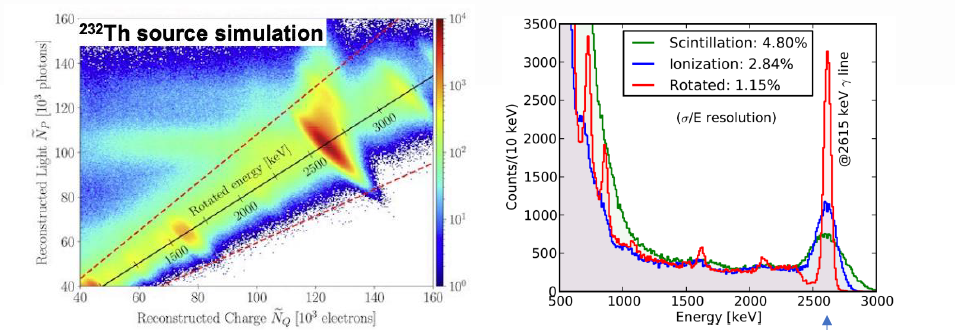
\includegraphics[scale=0.35]{scintioniexo.png}


%\column{0.40\textwidth}
$\bullet~$ Using anti-correlation between scintillation and ionisation yields a good combined energy resolution. EXO measured $\sigma = 1.15$\% at 2.6 MeV. This translates into  
$\sigma_{FWHM} = 3.5$\% at \qbb.  

%\end{columns}
\end{frame}

%%%
\begin{frame}{Topology in LXe}
\begin{columns}
\column{0.50\textwidth}
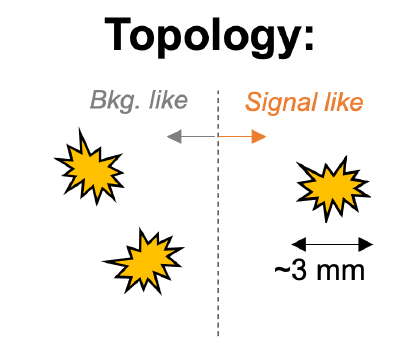
\includegraphics[scale=0.35]{exoTopo.png}


\column{0.50\textwidth}
$\bullet~$ A LXe TPC has the capability to separate single-site from multi-site events.  

$\bullet~$ This is extremely useful to reject pile-up events from low-energy gammas, but not so much for the critical backgrounds associated to \BI\ and \TL. In particular, in the case of \BI, the background event is a bona-fie photoelectric event, which produces a single-site. A LXe cannot separate between single and double electrons, and thus it depends on energy resolution to separate this background from signal.  

\end{columns}
\end{frame}
%%%

\begin{frame}{From EXO to nEXO}
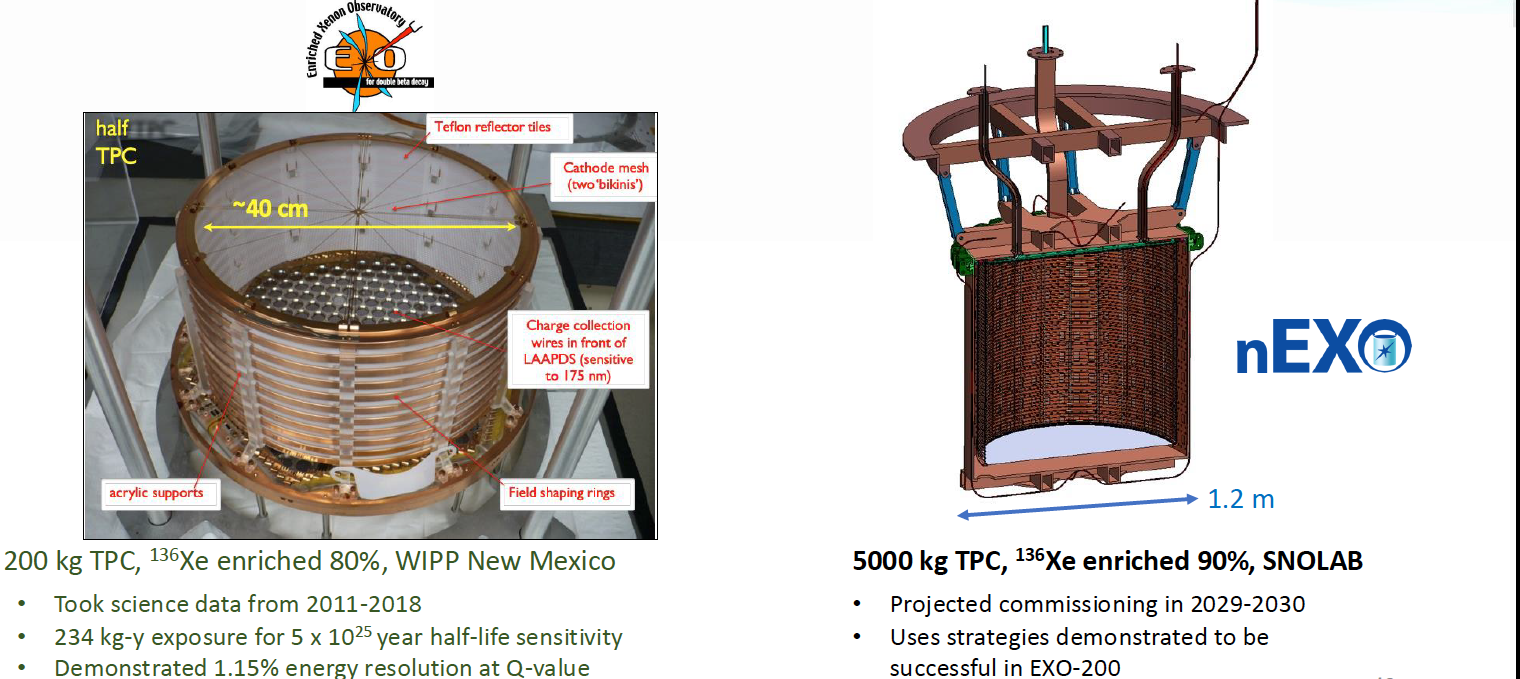
\includegraphics[scale=0.30]{exonexo.png}
\end{frame}

%%%

\begin{frame}{Double shell cryostat}
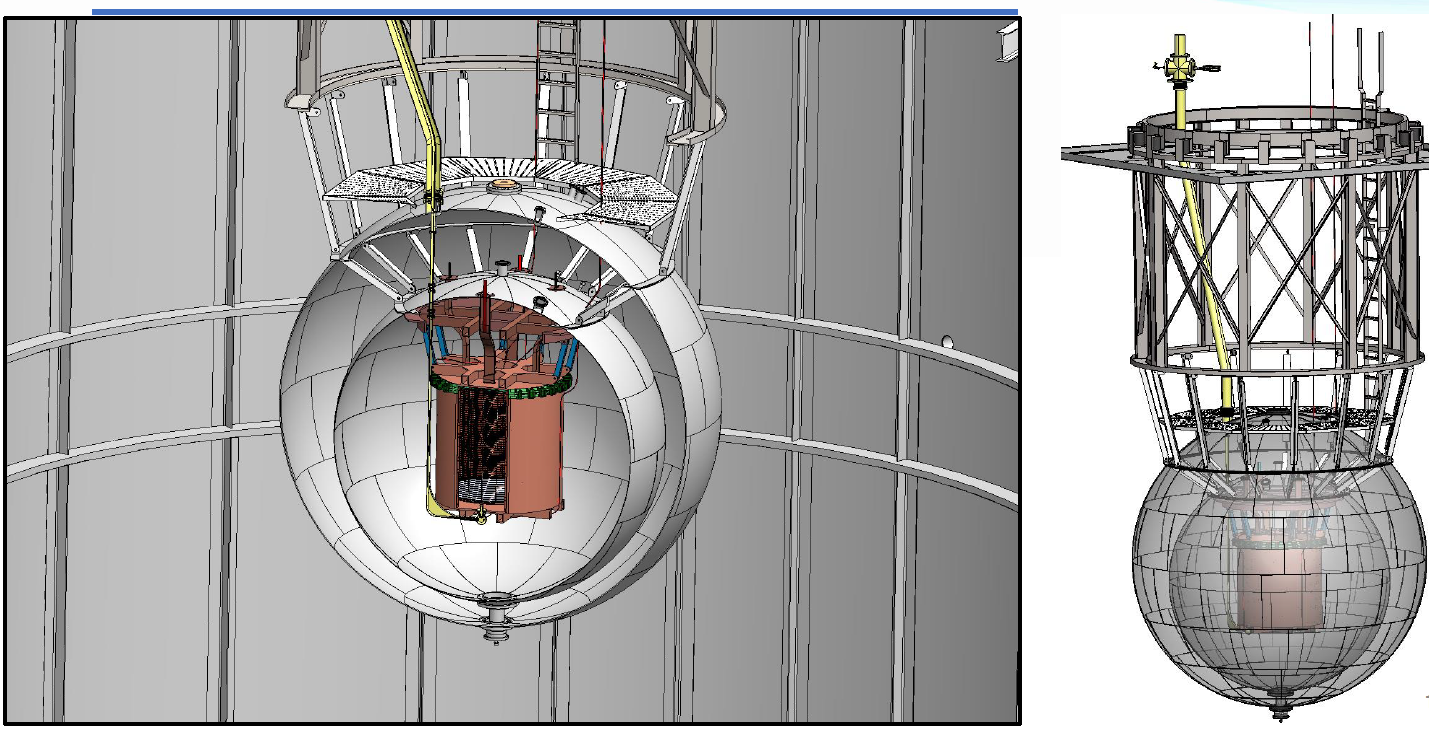
\includegraphics[scale=0.30]{nexoinsnow.png}
\end{frame}

%%%
\begin{frame}{nEXO would operate deep underground (SNOWLAB)}
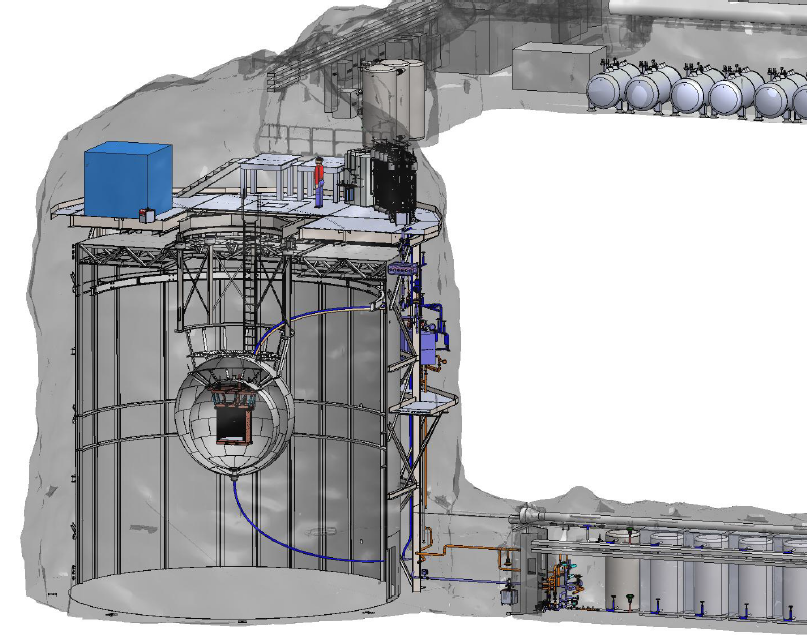
\includegraphics[scale=0.30]{nexosnowlab.png}
\end{frame}

%%%

\begin{frame}{Key elements of nEXO}
\begin{columns}
\column{0.50\textwidth}
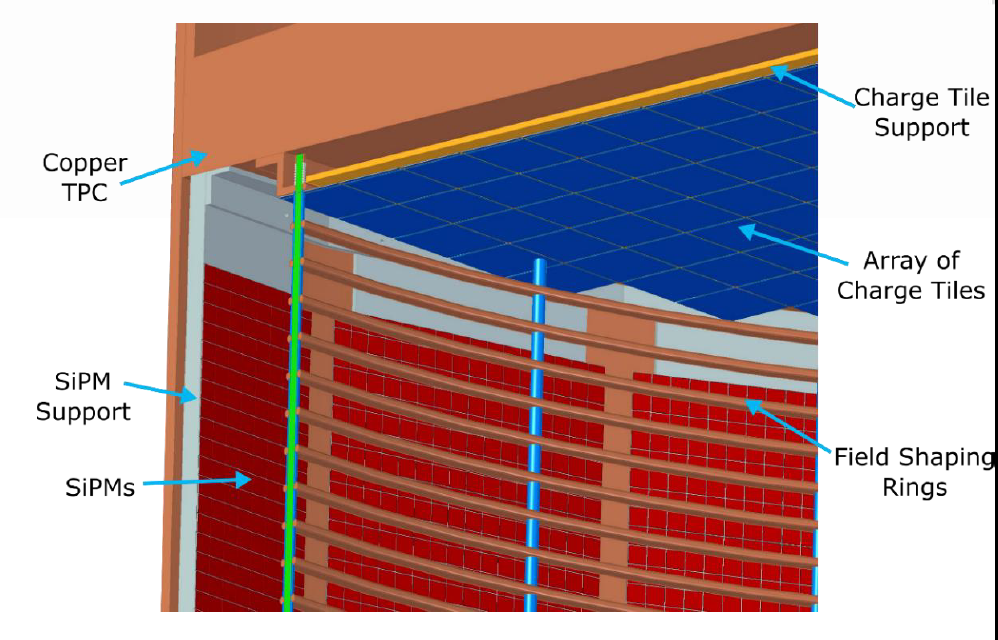
\includegraphics[scale=0.20]{nexokey.png}
\column{0.50\textwidth}
$\bullet~$ Key elements are very similar to those of NEXT-HD: The TPC vessel is made of ultra-pure copper, and the active elements are the charge-tiles (readout of ionisation) and photon detector system (readout of scintillation). The challenge in nEXO, like in NEXT is to achieve a level of radiopurity as high as possible in those components. 
\end{columns}
\end{frame}

%%%
\begin{frame}{Light readout}
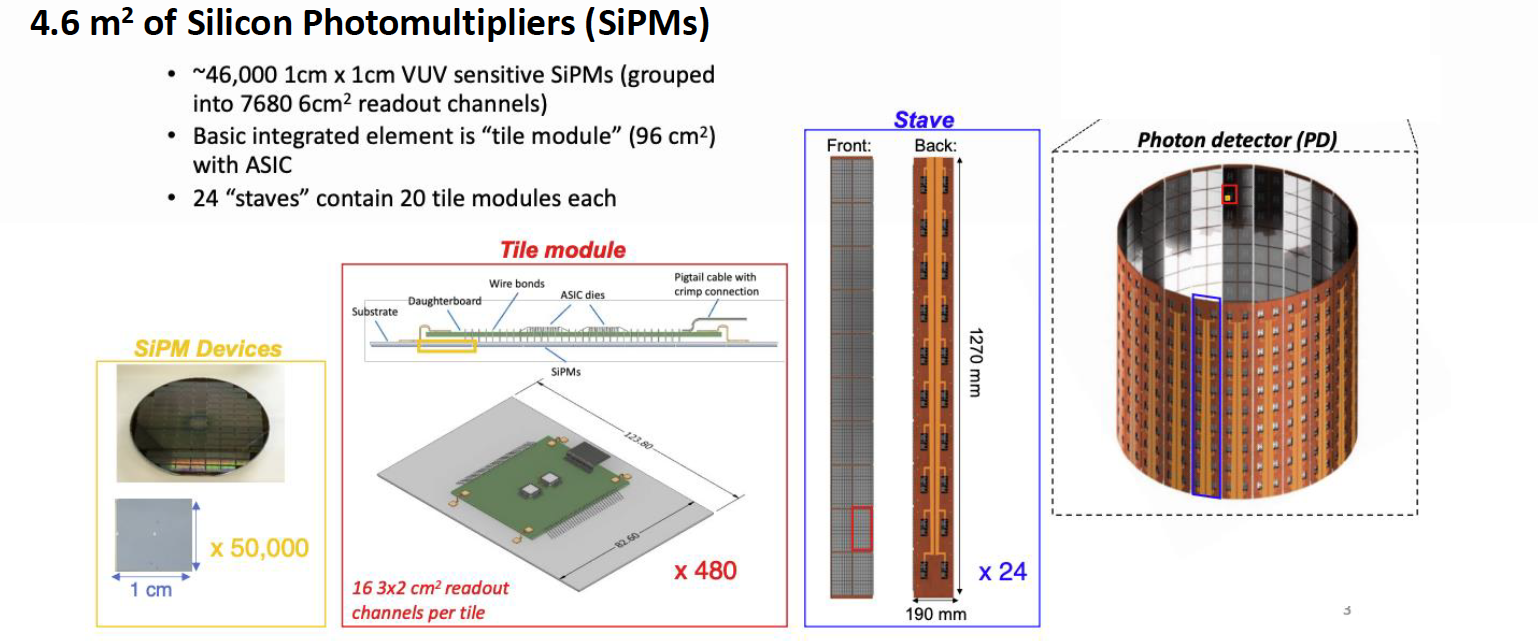
\includegraphics[scale=0.25]{nexoLightReadout.png}

$\bullet~$: In NEXT-HD, a ``dense tracking plane" could use similar ideas. The main advantage of nEXO is that the detector is cold, thus SiPMs DC is very small.  
\end{frame}

%%%

%%%
\begin{frame}{Charge detection system}
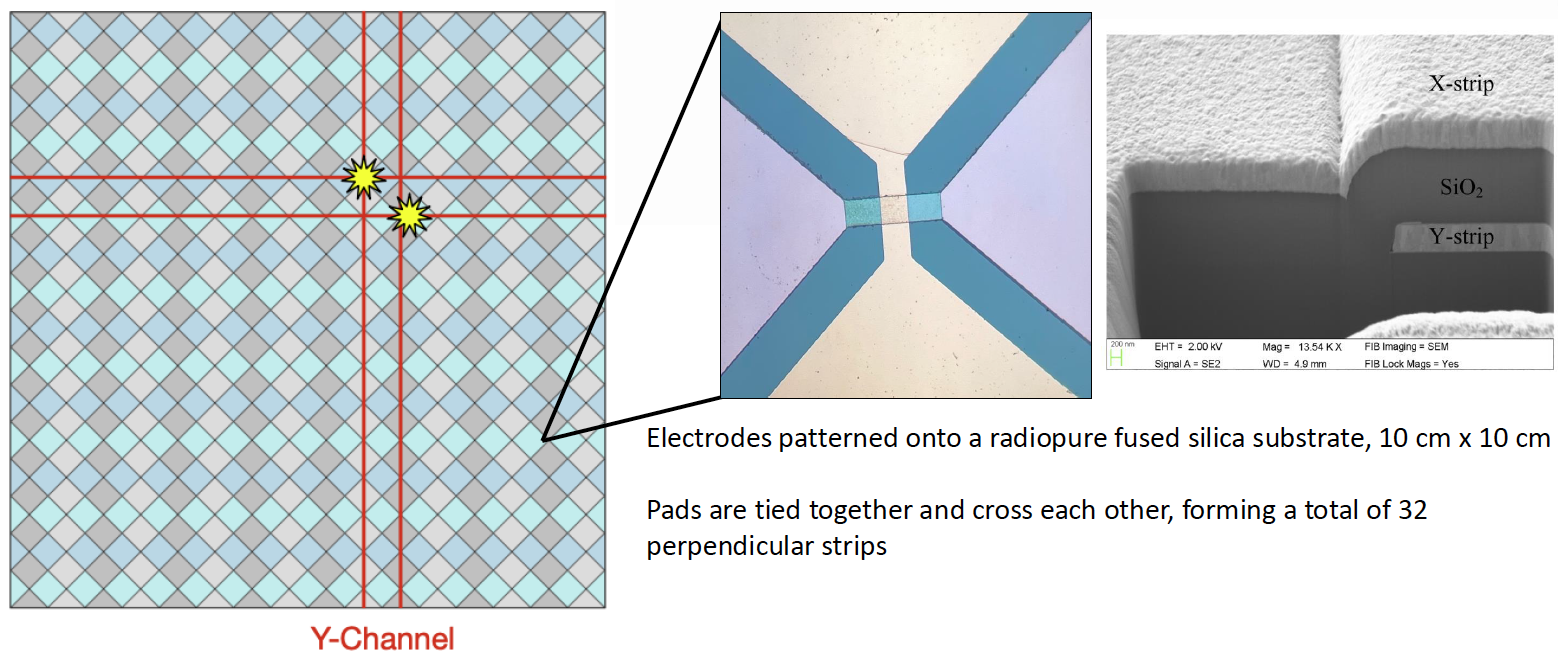
\includegraphics[scale=0.25]{nexocharge.png}
\end{frame}

%%%

\begin{frame}{Charge detection system}
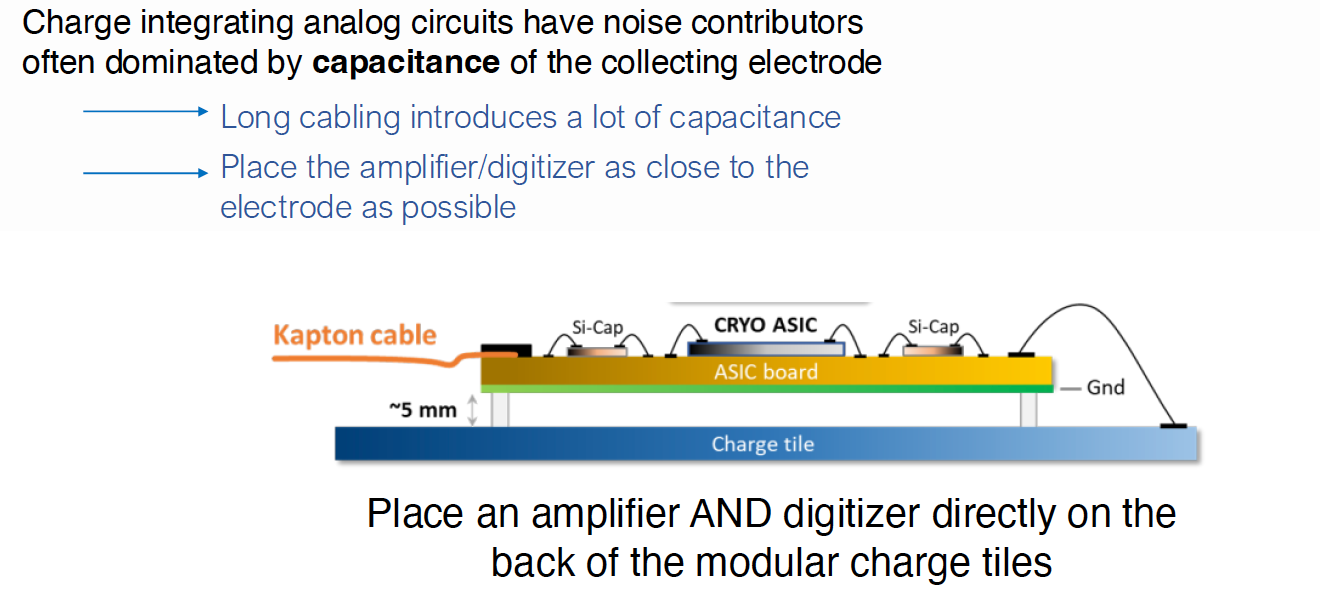
\includegraphics[scale=0.25]{chargeReadoutnexo.png}

$\bullet~$ Tradeoff: more material (electronics) near the active volume. 
\end{frame}

\begin{frame}{Electroformed copper vessel}
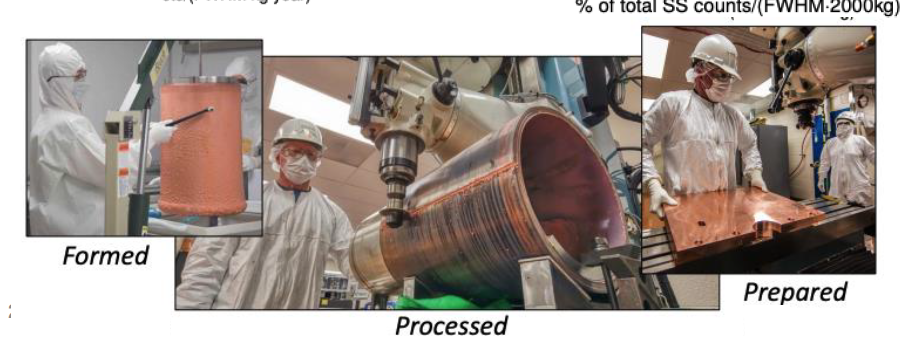
\includegraphics[scale=0.30]{electroformedcopper.png}

$\bullet~$ Useful technique for NEXT-HD too! ICS last radiation length made of same stuff than NEXO.  
\end{frame}

\begin{frame}{Field Cage}
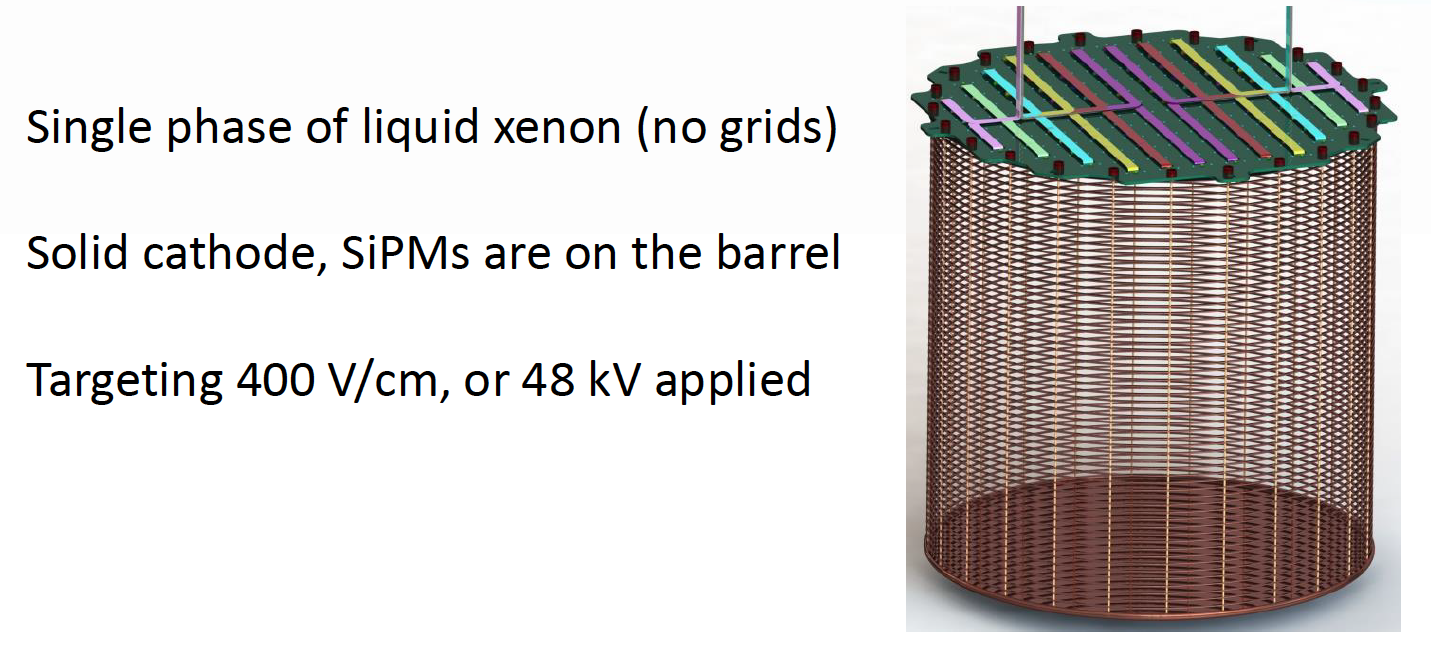
\includegraphics[scale=0.30]{nexoFieldCage.png}

$\bullet~$ Lots of common ground here between NEXT and nEXO (copper, resistors, grids, HV, etc.).  
\end{frame}

\begin{frame}{NEXT and nEXO handles}
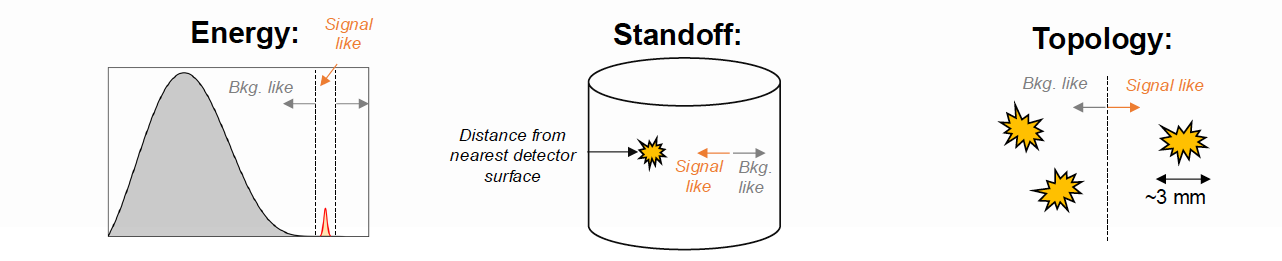
\includegraphics[scale=0.30]{nexoHandles.png}
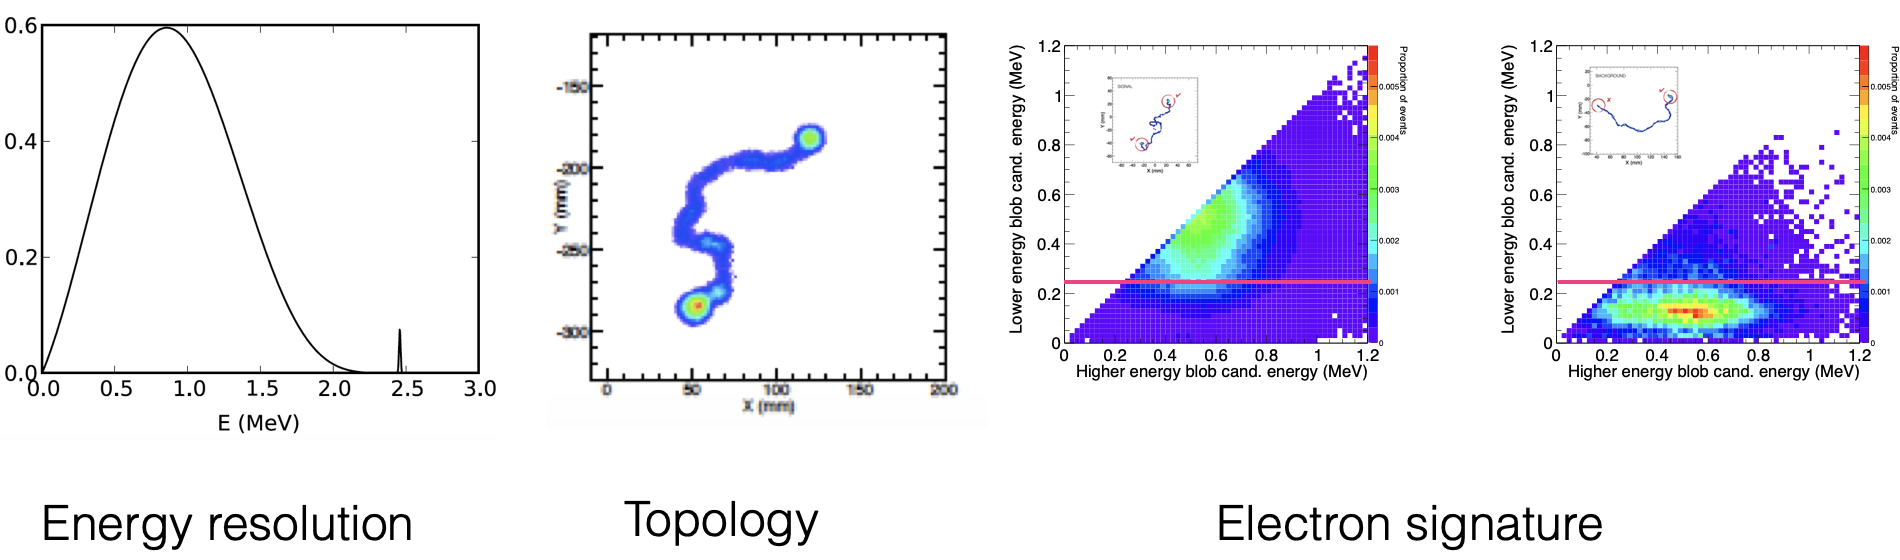
\includegraphics[scale=0.30]{nextSignatures.png}

$\bullet~$ (not so) Different strategies.   
\end{frame}



%\begin{frame}{Gamma transparency in GXe}
%\begin{columns}
%\column{0.50\textwidth}
%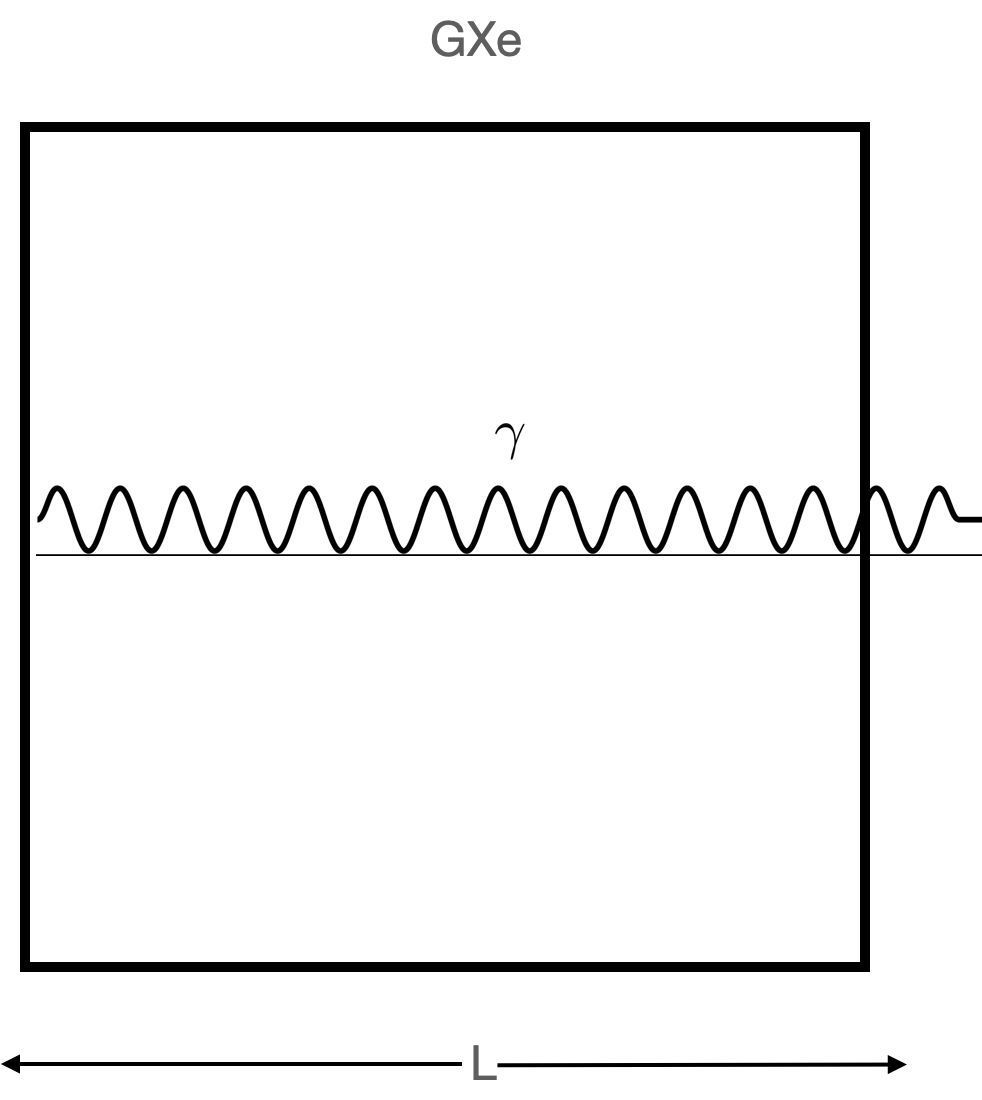
\includegraphics[scale=0.2]{nexttrans.png}
%
%$\bullet~$ Consider a cylinder of $L=D=1~ m^3$
%
%$\bullet~$ Condition of transparency is that $\gamma$ crosses the full volume
%\column{0.50\textwidth}
% $\mu/\rho = 4.8 \times 10^{-2}$~cm$^2$/g, gas STP, $\rho = 5.37$~g/m$^3$.
% 
% $\mu = 5.37 \times 4.8 \times 10^{-6} = 2.6 \times 10^{-5}$~m$^{-1}$.
% 
% Interacting: $ 1- e^{-\mu L} \sim 1 - e^{-2.6 \times 10^{-5}} = 2.6  \times 10^{-5}$
% 
% At 10 bar, $I \sim 2.6 \times 10^{-4}$
% 
% 
%\end{columns}
%\end{frame}



%%%
\end{document}